%-----------------------------------
% SECTION: Algorithm Specification
%-----------------------------------
\section{Algorithm Specification}
\label{sec:AlgorithmSpec}
Our authenticated encryption algorithm is based on a simplified duplex construction.
Padding and domain separation are assumed to be done at some higher level in the overall system if needed.
For this reason, it is sufficient to specify only the duplex parameters and the sponge function $f$.

%\begin{algorithm}
\caption*{\textbf{Algorithm} $f$ Round}
\label{alg:Algorithm}
\begin{algorithmic}
\Comment{Substitution Step}
\For{$x < 16$}
  \State $S[x] \gets Sbox(S[x])$
\EndFor
\If {$i > maxval$}
    \State $i \gets 0$
\Else 
    \State $blah$
\EndIf
\end{algorithmic}
\end{algorithm}



\subsection{Duplex Parameters}
We allow two key sizes: $128$ bits and $256$ bits.
Our construction uses a $512$-bit internal state, so we have $b = 512$.
The rate $r$ is $128$ bits for both key lengths, which means that the capacity $c$ is $384$.
Keeping the rate at a constant $128$ bits for both instantiations means that switching between key lengths is a trivial task.

The capacity $c = 384$ provides sufficient security against generic attacks for both $128$- and $256$-bit keys.
As explained in Section~\ref{sec:SpongeAndDuplex}, we know from \cite{Jovanovic2014_Beyond} that the generic security level is
\begin{equation*}
\mathrm{min}(2^{(r+c)/2}, 2^c, 2^{|K|}).
\end{equation*}
For a $128$-bit key, the generic security level is $2^{128}$.
For a $256$-bit key, the generic security level is $2^{256}$. 

\subsection{Permutation $f$}
Our underlying sponge function $f$ is a permutation and thus is invertible.
For compactness, we specify only the forward permutation here as the inverse is not required for practical purposes.

The permutation consists of a number of rounds.
Each round can be represented as the composition of several subfunctions or \emph{steps}: a substitution, a bitwise permutation, a mixing layer, and the addition of a round constant.

\subsubsection{Substitution Step}
The substitution step is a bricklayer permutation that uses $32$ identical, bijective $16 \times 16$ S-boxes.
This step is the main source of confusion within the permutation.
Furthermore, it is the only nonlinear step, as is typical with many substitution-based symmetric key algorithms \cite{Stinson2006_CTAP}.

To the best of our knowledge this is the first cryptosytem to use such large S-boxes.
We believe that, at the time of writing, the largest S-boxes used in the literature are the $8 \times 8$ bijective S-boxes used by the Advanced Encryption Standard (AES) \cite{Daemen2002_DesignOfRijndael}\cite{NIST2001_FIPS-197}.

Our S-box is an AES-inspired design taken directly from Wood's thesis on the subject \cite{Wood2013_SboxThesis}.
The primary reason for using this particular class of $16$-bit S-boxes is that they are efficiently implementable in hardware.
Rather than being based on a random mapping, they are based on multiplicative inversion in a finite field followed by an affine transformation.
This allows us to implement a circuit which performs the field operations rather than use the corresponding (and prohibitively large) look-up table.

This S-box is based on multiplicative inversion in $\gfsixteen / \left\langle p(x) \right\rangle$ where 
\begin{equation*}
p(x) = x^{16} + x^5 + x^3 + x + 1.
\end{equation*}
We represent an input to the S-box (and inverse S-box) as a $16$-bit column vector 
\begin{equation*}
x = 
\begin{pmatrix}
x_{15} & x_{14} & \ldots & x_1 & x_0
\end{pmatrix}^\mathrm{T},
\end{equation*}
where $x_{15}$ is the MSB.
Using this notation, the forward S-box function is given as
\begin{equation*}
\renewcommand{\arraystretch}{0.7} % Make it square
\mathbf{S}(x) = 
\begin{pmatrix}
0 & 0 & 1 & 0 & 0 & 0 & 0 & 1 & 0 & 0 & 1 & 1 & 1 & 1 & 1 & 0 \\
1 & 1 & 0 & 0 & 0 & 0 & 0 & 1 & 0 & 1 & 1 & 0 & 1 & 0 & 1 & 0 \\
1 & 1 & 0 & 0 & 1 & 0 & 1 & 1 & 0 & 1 & 0 & 1 & 0 & 0 & 1 & 1 \\
1 & 1 & 1 & 0 & 0 & 0 & 1 & 0 & 0 & 1 & 1 & 0 & 0 & 0 & 0 & 0 \\

1 & 1 & 0 & 0 & 0 & 1 & 1 & 0 & 0 & 1 & 1 & 1 & 1 & 0 & 1 & 1 \\
0 & 1 & 0 & 0 & 0 & 0 & 1 & 1 & 0 & 1 & 1 & 1 & 1 & 1 & 0 & 1 \\
0 & 0 & 1 & 0 & 1 & 0 & 1 & 0 & 1 & 1 & 0 & 0 & 1 & 1 & 0 & 0 \\
1 & 0 & 1 & 1 & 1 & 0 & 1 & 1 & 0 & 0 & 0 & 1 & 0 & 1 & 1 & 1 \\

0 & 1 & 0 & 0 & 0 & 0 & 0 & 0 & 1 & 0 & 0 & 1 & 1 & 1 & 0 & 1 \\
1 & 0 & 1 & 1 & 0 & 0 & 0 & 1 & 0 & 0 & 1 & 0 & 1 & 0 & 0 & 0 \\
1 & 0 & 1 & 0 & 0 & 1 & 1 & 1 & 0 & 0 & 1 & 1 & 0 & 1 & 0 & 0 \\
1 & 0 & 1 & 1 & 1 & 0 & 1 & 1 & 1 & 1 & 0 & 1 & 1 & 0 & 0 & 1 \\

1 & 0 & 1 & 0 & 0 & 1 & 0 & 1 & 1 & 0 & 0 & 1 & 0 & 0 & 0 & 1 \\
0 & 1 & 0 & 0 & 0 & 1 & 1 & 1 & 1 & 0 & 0 & 0 & 0 & 0 & 0 & 1 \\
1 & 0 & 0 & 0 & 1 & 1 & 0 & 1 & 0 & 1 & 1 & 1 & 1 & 0 & 0 & 0 \\
1 & 1 & 0 & 1 & 0 & 1 & 1 & 0 & 1 & 0 & 0 & 1 & 1 & 0 & 0 & 0 \\
\end{pmatrix}
\begin{pmatrix}
x_{15} \\
x_{14} \\
x_{13} \\
x_{12} \\
x_{11} \\
x_{10} \\
x_{9} \\
x_{8} \\
x_{7} \\
x_{6} \\
x_{5} \\
x_{4} \\
x_{3} \\
x_{2} \\
x_{1} \\
x_{0} \\
\end{pmatrix}
^{-1}
\oplus
\begin{pmatrix}
0 \\
1 \\
0 \\
0 \\
0 \\
1 \\
0 \\
1 \\
1 \\
0 \\
1 \\
1 \\
0 \\
1 \\
1 \\
1 \\
\end{pmatrix}.
\end{equation*}

A hardware implementation for this particular S-box requires just $1238$ XOR gates and $144$ AND gates.

\subsubsection{Bitwise Permutation Step}
Bitwise permutations are easily implementable in hardware via a simple rerouting of wires.
Compared to a permutation on the words of the state, a bitwise permutation intuitively provides much better diffusion.
The bitwise permutation step is the main source of long-range (i.e.\ across the entire state) diffusion in the algorithm.

The bitwise permutation also helps maximize the minimum number of active S-boxes by being subject to certain constraints.
We use a permutation that satisfies the following properties:
\begin{enumerate}
\item All outputs of a given S-box go to $16$ different mixers
\item The permutation is a \emph{derangement}; it has no fixed points
\item High order; it does not repeat within the number of rounds
\item No low order bits; the order of any bit equals the order of the overall permutation
\item Easily definable by some affine function
\end{enumerate}
There is obviously no cryptographic significance to how ``easy'' it is to express a bitwise permutation.
This is merely to cut down on the search space and to avoid having to provide a table with $512$ entries to express the permutation.
The \emph{order} of a bitwise permutation is the number of times it must be applied before it ends up in its original orientation.
A particular bit in a bitwise permutation also has the notion of order and a bit of low order is one that returns to its original position before the entire permutation begins to cycle.
If a bit has order zero, it is unaffected by the bitwise permutation and is called a \emph{fixed point}.

We chose the following permutation to use for our algorithm since it is the first function to satisfy all properties:
\begin{equation*}
\pi(x) = 31x + 15 \bmod{512}
\end{equation*}
This bitwise permutation has order $32$.
For a complete listing of all bitwise permutations that satisfy our requirements, refer to Appendix~\ref{appx:BitwisePermutations}.

\subsubsection{Mix Step}
The purpose of the mix step is to provide local diffusion (i.e.\ across two words) and increase the linear and differential branch numbers of a round from two to three.
We use a mixer based on multiplication by a $2 \times 2$ matrix in \gfsixteen modulo the irreducible polynomial
\begin{equation*}
p(x) = x^{16} + x^5 + x^3 + x^2 + 1.
\end{equation*}
The mixer takes two words $A$ and $B$ as input and produces outputs $A'$ and $B'$ as follows:
\begin{equation*}
\begin{pmatrix}
A' \\ B'
\end{pmatrix}
=
\begin{pmatrix}
1 & x \\ x & x + 1
\end{pmatrix}
\begin{pmatrix}
A \\ B
\end{pmatrix}
\end{equation*}
The MSB of each word is taken as the leftmost bit and is represented by $x^{15}$. 

The forward mixer is efficiently implementable in hardware.
Figure~\ref{fig:MixerMatrix} shows how this matrix multiplication is implemented.
The $x*$ operation is a multiplication by $x$ in \gfsixteen.
Its implementation, which is shown in Figure~\ref{fig:xTimes}, is very simple. 

\begin{figure}[ht]
\centering
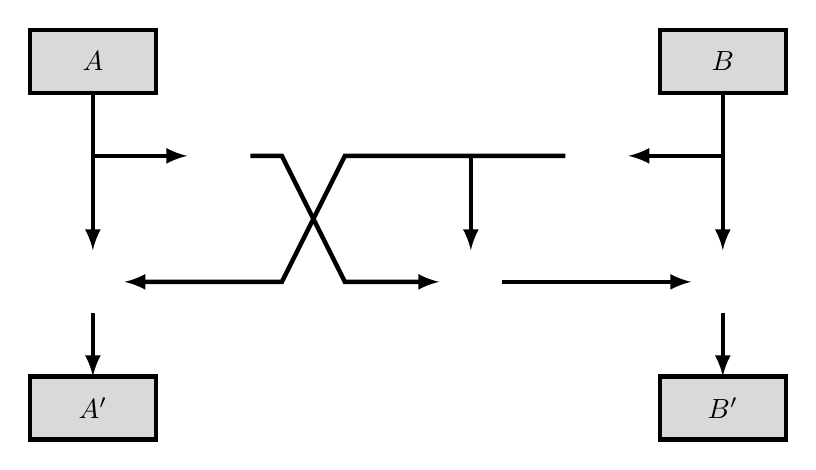
\begin{tikzpicture}[xscale=0.8,yscale=0.8,>=latex,ultra thick]
% Reference grid (temporary)
%\draw[help lines] (0,0) grid (16,16);

% Inputs
\draw[fill=gray!30] (0,15) rectangle (2,14) node[midway] {$A$};
\draw[fill=gray!30] (10,15) rectangle (12,14) node[midway] {$B$};

\draw[->] (1,14) to (1, 11.5);
\draw[->] (1,13) to (2.5, 13);

\draw[->] (11,14) to (11, 11.5);
\draw[->] (11,13) to (9.5, 13); 

\drawxTimes{3}{13}
\drawxTimes{9}{13}

\drawXOR{1}{11}
\drawXOR{11}{11}
\drawXOR{7}{11}

\draw[->] (3.5,13) to (4,13) to (5,11) to (6.5,11);
\draw[->] (8.5,13) to (5,13) to (4,11) to (1.5,11); 
\draw[->] (7,13) to (7,11.5);
\draw[->] (7.5,11) to (10.5,11);

\draw[->] (1,10.5) to (1,9.5);
\draw[->] (11,10.5) to (11,9.5);

% Outputs
\draw[fill=gray!30] (0,9.5) rectangle (2,8.5) node[midway] {$A'$};
\draw[fill=gray!30] (10,9.5) rectangle (12,8.5) node[midway] {$B'$};

\end{tikzpicture}

\caption{Hardware implementation of the forward mixer function.}
\label{fig:MixerMatrix}
\end{figure}

\begin{figure}[ht]
\centering
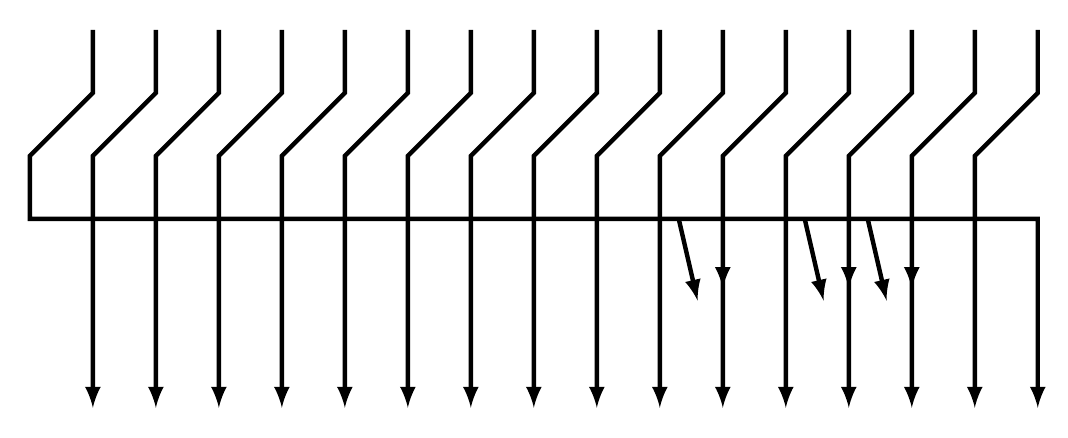
\begin{tikzpicture}[xscale=0.8,yscale=0.8,>=latex,ultra thick]
% Reference grid (temporary)
%\draw[help lines] (0,0) grid (24,24);

\draw[->] (1,24) to (1,23) to (0,22) to (0, 21)
    to (16, 21) to (16, 18);
\foreach \i in {2,...,16} {
    \draw[->] (\i,24) to (\i,23) to (\i-1,22) to (\i-1, 18);
}
\draw[->] (10.3,21) to (10.6,19.7);
\draw[->] (11,21) to (11,19.9);
\drawXOR{11}{19.5}
\draw[->] (12.3,21) to (12.6,19.7);
\draw[->] (13,21) to (13,19.9);
\drawXOR{13}{19.5}
\draw[->] (13.3,21) to (13.6,19.7);
\draw[->] (14,21) to (14,19.9);
\drawXOR{14}{19.5}
\end{tikzpicture}

\caption{Hardware implementation of the $x*$ function. The leftmost bit is the MSB.}
\label{fig:xTimes}
\end{figure}

\subsubsection{Add Round Constant Step}
This step consists of adding a $512$-bit value to the state using bitwise XOR in order to disrupt symmetry and prevent slide attacks.
The round constant $RC_i$ for round $i$ is given by the formula
\begin{equation*}
RC_i = \mathbf{SHA3\textbf{-}512}(\mathbf{ASCII}(i)),
\end{equation*}
where $\mathbf{ASCII}(i)$ is a function that provides the one or two byte ASCII representation of $i$ and $\mathbf{SHA3\textbf{-}512}$ is the SHA-3 hash function that outputs a $512$-bit message digest. 

\subsection{Number of Rounds}
This algorithm uses $10$ rounds for a $128$-bit key and $16$ rounds for a $256$-bit key.
The number of rounds is determined, as is typical with block ciphers and permutations, by calculating the number needed for resistance to linear and differential cryptanalysis and adding some buffer to increase the security margin. 
For a more in-depth treatment, refer to Section~\ref{sec:Cryptanalysis}.

\subsection{Customization}
While a specific instantiation is specified here, our algorithm is highly customizable within our security margin.
This could be useful in the case that different users want unique, proprietary algorithms.
We list several possible customizations here.

\subsubsection{State Initialization}
In the given specification, the inner state (like the outer state) is initialized to zero.
This is not a requirement; indeed, the inner state could be initialized to any $384$-bit value.
Each user could generate their own unique value to set during the initialization phase.
This happens before the first mute calls that absorb the key.

\subsubsection{S-boxes}
The AES-inspired S-box used here is efficiently implementable in hardware.
There are certainly many other cryptographically secure $16$-bit S-boxes, but randomly generated ones may not be suitable for hardware implementation due to size constraints.
This is an area for further research.
Still, several other AES-like $16$-bit S-boxes are presented in \cite{Wood2013_SboxThesis}.
Any new S-box introduced into the algorithm shall be analyzed to determine its linear and differential characteristics and the number of rounds should be adjusted accordingly if necessary.
This analysis can easily be performed using the tools mentioned in Section~\ref{sec:Cryptanalysis}.

\subsubsection{Bitwise Permutations}
The bitwise permutation provided in this algorithm specification is one of many that satisfies the constraints we impose.
We provide all suitable bitwise permutations in Appendix~\ref{appx:BitwisePermutations}.
Users may select any of these without need for further cryptanalysis.

\subsubsection{Mixers}
Our mixer is based on a specific $2 \times 2$ matrix multiplication in \gfsixteen modulo a specific irreducible polynomial $p(x)$.
Many matrices are expected to satisfy the constraints that we impose.
These constraints are:
\begin{enumerate}
\item The $2 \times 2$ matrix should be invertible in $\gfsixteen /\left\langle p(x) \right\rangle$
\item The matrix should have differential and linear branch number equal to three (the maximum possible)
\end{enumerate}
Like the addition of a new S-box, any new matrix introduced to the algorithm should be analyzed to ensure it meets these constraints.
This analysis can also easily be performed using the tools mentioned in Section~\ref{sec:Cryptanalysis}.

\subsubsection{Round Constants}
The round constants presented here are based on SHA-3 hash values.
However, they could be any values that satisfy the following constraints.
Round constants should be:
\begin{enumerate}
\item Unique for each round; to prevent against slide attacks
\item Random, pseudorandom, or highly asymmetric; to reduce symmetry in the state
\end{enumerate}
The round constants are not expected to have any cryptographic significance outside of this.
Different users can generate their own unique set of round constants without difficulty.

